% Chapter 2

\chapter{Films polim\'ericos} % Main chapter title

\label{Chapter2} % For referencing the chapter elsewhere, use \ref{Chapter1}

%\section{papers of films}


Los films polim\'ericos o hidrogeles  consisten en una red de pol\'imeros entrecruzados altamente hidratados, generalmente biocompatibles, dependendiendo de su composici\'on qu\'imca. El ambiente acuoso dentro de los hidrogeles puede proteger a las prote\'inas de la desnaturalización y la agregaci\'on [11e13], mientras permanecen activas y estructuradas cuando se liberan de los hidrogeles [14]. En la administraci\'on oral de f\'armacos, los hidrogeles con respuesta de pH se han investigado en gran medida como veh\'iculos funcionales que pueden encapsular y administrar prote\'inas, evitando su degradaci\'on en el entorno gastrointestinal [15-17].


En este capitulo mostraremos un estudio  de estos sistemas polim\'ericos haciendo uso de de la te\'oria molecular.



\section{Te\'oria Molecular en films polim\'ericos}


Este m\'etodo consiste en minimizar una energ\'ia libre generalizada que incluye toda la termodinamica relevante que engloba los procesos del film contacto con una soluci\'on.
Para tal fin se necesita de una descripci\'on molecular de grano grueso de las diferentes especies qu\'imicas que componen el sistema.
Dicha descripci\'on incluye forma, tama\~no, distribuci\'on de carga (si los hubiese) y estado de protonaci\'on de cada componente molecular en los casos que corresponda.
En esta primera instancia describiremos la fisicoqu\'imica de un film  se encuentra en  equilibrio con una solución acuosa, la tiene una composición  definida externamente.
Es decir, el pH, la concentración de sal y la concentraci\'on de adsorbatos son variables independientes.

Para esto nos valdremos de una  red polim\'erica que da estructura a nuestro film, que posee distintos tipos de segmentos: una unidad sensible al pH, en particular consideraremos un film polim\'erico compuesto por unidades \'acidad de \'acido metacr\'ilico ($MAA$).

Este film est\'a  se encuentra en equilibrio con una soluci\'on con una temperatura, pH y concentraci\'on de sal definidas. Adem\'as vamos a considerar que en dicha soluci\'on hayun adsorbato: una prote\'ina.
El uso de una prote\'ina modelo como adsorbato nos beneficia dado que poseen disitinto tipos de amino\'acidos con lo cual la descripci\'on de la misma puede ser usada para otros adsorbatos. 


Considerando los aspectos anteriores es posible definir una energ\'ia libre:

\begin{align}
 	F = -TS_{mez} -TS_{conf,nw} + F_{chem,nw} + F_{chem,pro} + U_{elec} + U_{ste} + U_{VDW}
 	\label{eq:libre-film}
\end{align}
 
\noindent En donde $S_{mez}$ es la entrop\'ia de traslaci\'on ( y de mezcla) de las especies libres en la soluci\'on: mol\'eculas de agua (H$_2$O), y sus respectivos iones:  hidronio (H$_3$O$^+$), e hidr\'oxido (OH$^- $), cationes y aniones de sal y nuestra prote\'ina modelo.
Aqu\'i, consideramos una sal monovalente, NaCl, la cual est\'a completamente disociada en sus  iones cloruro (Cl$^-$) y sodio ($Na^+$). 

$S_{conf,nw}$ representa la entrop\'ia conformacional que resulta de la flexibilidad de la red de polim\'erica, la cual viene dada por todas las conformaciones diferentes que puede asumir la misma.

$F_{chem,nw}$, es la energ\'ia qu\'imica libre que describe el equilibrio entre las especies protonadas y desprotonadas de unidades funcionales (\'acidas/b\'asicas), para nuestro film solo se consideran unidades \'acidas.

De manera similar, $F_{chem,pro}$ describe la protonaci\'on de residuos titulables de la prote\'ina.

$U_{elec}$ y $U_{ste}$ representan, respectivamente, las interacciones electrost\'aticas y las repulsiones est\'ericas.
Las interacciones de Van der Waals son representadas en $U_{VdW}$.


Las expresiones explicitas de la ecuaci\'on \ref{eq:libre-film} las describimos acontinuaci\'on.

Como primer termino tenemos la entrop\'ia de mezcla de  las especies mobiles, entre ellas consideramos a nuestra prote\'ina modelo:

\begin{align}
	\begin{aligned}
		-\frac{S_{mez}}{k_B}= &A\sum_{\gamma}\int_0^\infty{dz\rho_\gamma(z)\left(\ln \left(\rho_\gamma (z)v_w\right) -1 + \beta\mu^0_\gamma\right)} \\
		&+ A\sum_{\theta}\int_0^\infty{dz\rho_{pro}(\theta,z)\left(\ln \left(\rho_{pro}(\theta,z)\right) -1 + \beta\mu^0_{pro} \right)}
	\end{aligned}
\end{align}

\noindent en donde $\frac{1}{k_B T}$, y $k_B$ es la constante de Boltzmann, $T$ es la temperatura absoluta del sistema. La variable $z$ es la coordenada que mide la distancia a la superficie de soporte de nuestro film, el \'ara total de esta superficies es $A$. $\rho_\gamma(z)$ y $\mu_\gamma$ es densidad local, a un $z$ dado, y potencial qu\'imico estadar de la especie $\gamma$ respectivamente.
El subinidice $\gamma$ toma en cuenta la mol\'ecula de agua y sus respectivos ione (hidronio e hidr\'oxido), adem'as de los iones provenientes de la sal ($K^+$ y $Cl^-$). 


El segundo t\'ermino de esta ecuaci\'on corresponde a la entrop\'ia de mezcla de la prote\'ina. $\rho_{pro}(\theta,z)$ es la densidad local de la prote\'ina en la conformaci\'on $\theta$. Es decir $\theta$ recorre sobre las configuraciones de la misma.
Esta conformaciones incluyen rotaciones espaciales de la prote\'ina.
De este modo la densidad local media de la prote\'ia puede expresarse como:


\begin{align}
	\left<\rho_{pro}(z)\right> = \sum_\theta{\rho_{pro}(\theta,z)}
\end{align}


La entrop\'ia conformational que resutla de la flexibilidad de la red polim\'erica de nuestro film se representa en $S_{conf, nw}$, esta tiene en cuenta todas las configuraciones de un set $\{\alpha\}$.

\begin{equation}
	\frac{S_{conf,nw}}{k_B} = - \sum_{\alpha}{P(\alpha)\ln P(\alpha)}
\end{equation}

\noindent en donce $P(\alpha)$ denota la probabilidad de que el film se encuentre en la configuraci\'on $\alpha$.

El siguiente t\'ermino de eq \ref{eq:libre-film} describe  la energ\'ia libre dada por  el equilibrio \'acido-base de los segmentos de MAA que componen nuestra red. 

\begin{align}
	\begin{aligned}
		\beta F_{chem,nw} &= A\int_0^\infty dz \frac{\left<\phi_{MAA}(z)\right>}{v_{MAA}} \left[f(z)(\ln f(z)+ \beta\mu^0_{MAA^-})\right.\\
		&\left.+(1-f(z))(\ln (1-f(z))+\beta\mu^0_{MAAH})\right]    
	\end{aligned}
\end{align} 

\noindent en donde $f(z)$ es el grado de carga de los segmentos de MAA entre las capaz $z$ y $z + dz$. 
$\mu^0_{MAA^-}$ y $\mu^0_{MAAH}$ son los potenciales qu\'imoc estandar  de las especies protonadas y desprotonadas respectivamente.
$v_{MAA}$ es el volumen molecular del segmento de MAA. El subindice $i$ recorre los tipos de segmentos que componen al film ( en nuestro caso $i = MAA$), pero en forma generica se define:

\begin{align}
	\left< \phi_i(z)\right> = \sum_\alpha{P(\alpha)\phi_i(\alpha,z)}
\end{align}
\noindent en el cual $\phi_i(\alpha,z)$  es el ensamble promedio. El cual es una variable de entrada que cuantifica la fracci\'on de volumen ocupado en una capa $z$ cuando la red se encuentra en la conformaci\'on $\alpha$.


%%%%%%%%%%%%%%%%%%%
El equilibrio qu\'imico de las unidades titulables de la prote\'ina es considerada en el siguiente t\'ermino de la energ\'ia libre:

\begin{align}
	\begin{aligned}
		\beta F_{chem,pro} = A\int_0^\infty dz& \sum_\tau \left<\rho_{pro,\tau}(z)\right> \left[g_\tau(z)(\ln g_\tau(z)+ \beta\mu^0_{\tau p})\right.\\
		&\qquad\left.+(1-g_\tau(z))(\ln (1-g_\tau(z))+\beta\mu^0_{\tau d})\right]   
	\end{aligned}
\end{align} 

\noindent en donde $\left<\rho_{pro,\tau}(z)\right>$ representa la densidad local promedio del segmento protonable $\tau$ de la prote\'ina.

Que se define como:
\begin{align}
	\left<\rho_{pro,\tau}(z)\right> = A\sum_\theta \int dz^\prime  \rho_{pro}(\theta,z^\prime)n_\tau(\theta,z^\prime, z)
	\label{eq:segments_pro_si}
\end{align}
\noindent en donde $n_\tau(\theta,r^\prime, r)$ es un par\'ametro de entrada que nos da el n\'umero de segmentos $\tau$ entre las capas $z$ and $z+ dz$ cuando el centro de masa de la prote\'ina se encuentra en el a configuraci\'on $\theta$ y en la posici\'on $z^\prime$.

Las unidades titulables pueden estar en esta protonado $\tau p$ o desprotonado $\tau d$, los cuales poseen su potenciales qu\'imicos est\'andar $\mu^0_{\tau,p}$ y $\mu^0_{\tau,d}$ respectivamente. 
Adm\'as definimos el grado de asociaci\'on $g_\tau$ para segmento $\tau$ como:


\begin{enumerate}
	\item para unidades \'acidas: $g_\tau(r) = 1-f_\tau(r)$ ( las unidades $\tau$ se cargan negativamente)
	\item para unidades b\'asicas: $g_\tau(r) = f_\tau(r)$ (las  unidades $\tau$ se cargan positivamente  )
\end{enumerate}
en donde  $f_\tau(r)$ es el grado de disosiac\'on de cada segmento $\tau$.
%%%%%%%%%%

La energ\'ia electr\'ostatica se define como:
\begin{align}
	\begin{aligned}
		\beta U_{elecc}= A\int_0^\infty dz&\left[\left(\sum_{\gamma } {\rho_\gamma(z) q_\gamma + \sum_\tau{f_\tau(z) \left<\rho_{pro,\tau}(z)\right> q_\tau} +  f(z)\dfrac{\left<\phi_{MAA}(r)\right>}{v_{MAA}}q_{MAA}}\right)\beta\Psi(z) \right. \\ &\left.-\frac{1}{2}\beta\epsilon(\nabla\Psi(z))^2 \right]
	\end{aligned}
\end{align} 

\noindent en donde $\Psi(z)$ es el potencial elestr\'ostatico dependiente de la posici\'on, $\epsilon$ es la constante de permitividad del medio, $q_\gamma$ es la carga correspondiente a la especiel m\'obil $\gamma$, $q_\tau$ es la carga que adquieren los segmentos titulables de la prote\'ina. Finalmente $q_{MAA}$ es la carga que adquiere el segmento de $MAA$ al desprotonarse.


En este contexto, la densidad de carga media es:

\begin{align}
	\left<\rho_q(z)\right> = \sum_{\gamma } {\rho_\gamma(z) q_\gamma + \sum_\tau{f_\tau(z) \left<\rho_{pro,\tau}(z)\right> q_\tau} +  f(z)\dfrac{\left<\phi_{MAA}(z)\right>}{v_{MAA}}q_{MAA}}
	\label{si:eq:rho_charge}
\end{align}
%%%%%%%%%%%%%%%%

La contribuci\'on siguiente en la energ\'ia libre viene dada por la repulsi\'on esterica entre  todos los segmentos que componen  el sistema. Esta contribuci\'on se incorpora a travez del siguiente restricci\'on:  

\begin{align}
	\begin{aligned}
		1=  {\left[\sum_{\gamma}\rho_\gamma(z) v_\gamma + \sum_\lambda{\left<\rho_{pro,\lambda}(z)\right>v_\lambda} + \sum_i{\left<\phi_i(z)\right>}\right]},~ \forall z
	\end{aligned}
	\label{si:eq:constraint}
\end{align}
\noindent en donde  $v_\lambda$ es el volumen molecular del segmento $\lambda$  en la prote\'ina.
$\left<\rho_{pro,\lambda}(z)\right>$ es definimo de la misma forma que en la eq.  \ref{eq:segments_pro_si}.
Cabe destacar que el subidice $\lambda$ considera a todos los segmentos de la prote\'ina, es decir $ \tau \in \lambda$.
El subindice $i$ tiene en cuenta los segmentos del film.

%%%%%%%%%%%%%%%
$U_{VdW}$ is the energy of the Van der Waals interaction ($VdW$). In this work it has been assumed that all segments have a hydrophilic character. Namely, $VdW$ interactions between different pair of segments, and those with water molecules are similar. As a result the net $VdW$ interaction energy represent an additive constant to the total free energy.
Thus, this contribution can be ignored.


To complete the gran potential of eq:semicano , the exchange of mobile species is taken into account:

The first two terms on the left side of the equation account for the chemical equilibrium of the mobile species $\gamma$ and of the proteins within the solution.
The last two terms consider the hydrogen ions from the protonatable segments of the protein and the MAA segments of the polymer network that makes up the nanogel.


\begin{align}
	\begin{aligned}
		\mu_\gamma N_\gamma + \mu_{pro} N_{pro} =\int_0^\infty drG(r)&\left[\sum_{\gamma }{\rho_\gamma(r)\mu_\gamma}
		+ \mu_{pro} \left<\rho_{pro}(r)\right> \right. \\
		& \left. +\mu_{H^+}\sum_{\tau}{g_\tau\left<\rho_{pro,\tau}(r)\right> } +\mu_{H^+}(1-f(r))\dfrac{\left<\phi_{MAA}(r)\right>}{v_{MAA}}\right]
	\end{aligned}
\end{align}


%%%%%%%%%%
The explicit form of the grand potential is expressed as:



\subsection{Respuesta al pH}
\textbf{pH} \\
Hidrogeles  compuestos por cadenas de poli\'acidos son sensibles a los cambios de pH. Esta respuesta se debe a la equilibrio qu\'imico de protonaci\'on/desprotonaci\'on de las unidades \'acidas que componen la red. 
Para enteneder el funcionamiento de esta respuesta recordaremos algunos conceptos sobre el comportamiento \'acido/base de moleculas bajo condiciones ideales. 
Estos conceptos nos serviran para entener el equilibrio que ocurre cuando se confinan los monomeros en una red polim\'erica. Los mismos principios ser\'a utilizados para los sistemas  de estudio de los pr\'oximos capitulos.

Si consideramos una soluci\'on diluida de moleculas titulables, estas pueden exhibir dos estados posibles: protonado o desprotonado. En este sentido se define el grado de disoción, $f_d$, el cual  proporciona la fraci\'on de moleculas que se encuentran en estado desprotonado:


\begin{equation}
    f_d = \frac{1}{1+10^{pk_a -pH}}
    \label{eq:diso}
\end{equation}

si consideramos moleculas \'acidas su estado protonado no posee carga, es  neutro, por otro lado su estado desprotonado posee carga. 
Al considerar esto el grado de disociaci\'on, adem\'as nos indica el grado de carga de estas moleculas, $f_c$.
Para molecualas b\'asicas su estado de carga es contrario a las moleculas \'acidas, en consecuencia el grado de carga viene dado por: $f_c =1- f_d$.

En soluciones diluidas el grado de disociaci\'on $f_d$ (y el de carga $f_c$) son completamente determinados por el pH de la soluci\'on y el $pK_a$ intrinseco del par \'acido/base. 
Cuando el pH =$pK_a$ la mitad de los grupos titulables se encuentran en disosiados ($f_d = 0.5$). Para valores de $\pm 1$ coresponden a estados con 90\% y 10\% de disociaci\'on respectivamente.
Es decir, cuando el pH aumenta alrededor del pKa, la transici\'on del 10 al 90 \% de desprotonaci\'on ocurre dentro de dos unidades de pH de la soluci\'on ideal. 

Estas consideraciones de soluci\'on ideal usualmente se utilizan para estimar el grado de carga de las unidades \'acidas dentro de cadenas pol\'imerias. Sin embargo, este comportamiento es diferente para sistemas  en confinamiento. Las unidades  protonables forman parte de una red polim\'erica son un ejemplo de ello, lo cual modifica significativamente su comportamiento de protonaci\'on.


\textbf{Red polim\'erica} \\

A continuaci\'on describiremos el comportamiento de estos sistemas confinados, hidrogeles sensibles al pH.  A diferencia de las soluciones diluidas, las unidades \'acidas en una red de pol\'imeros experimentan repulsiones electrost\'aticas cuando estas se encuentran cargadas. Para reducir la fuerza de las repulsiones dentro de la red, estos grupos se disocian significativamente menos que en condiciones ideales. En la figura \ref{fig:degree-film} se ilustra este comportamiento y muestra el grado medio de carga de los segmentos de una pel\'icula de hidrogel de \'acido poli(metacr\'ilico) (PMAA), que est\'a en contacto con soluciones que tienen diferentes concentraciones de sal.
\begin{figure}
    \centering
    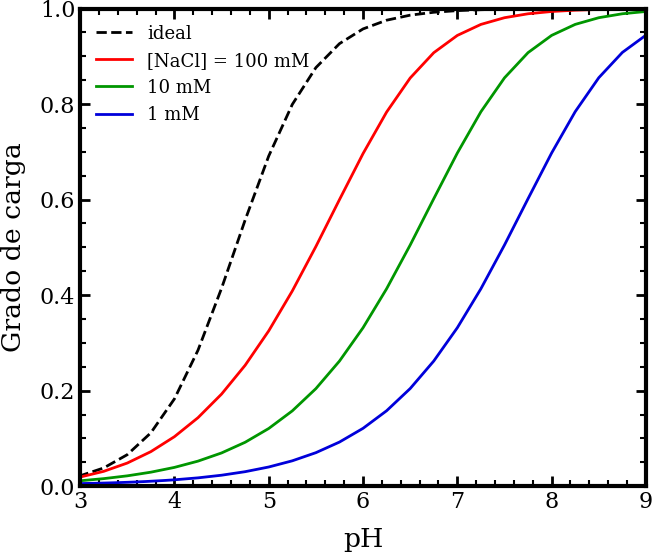
\includegraphics[width=0.9\textwidth]{Figures/graph-film/charge_degree-film.png}
    \caption{Grado de carga del gel como funci\'on del pH. Grado de carga para un monomero aislado en presentado en curva a rayas, se compara para diferentes concentraciones de sal, a mayor concentraci\'on salina m\'as nos acercamos al sistema ideal.}
    \label{fig:degree-film}
\end{figure}



A un pH dado es significativamente menos probable que se cargue una unidad \'acida de la red de lo que se espera seg\'un las consideraciones ideales. La concentraci\'on de sal de la soluci\'on resulta ser una variable cr\'itica que modula este comportamiento de regulación de carga.

A una salinidad relativamente alta, la cantidad de los contraiones dentro del hidrogel crece, lo que da como resultado el apantallamiento de interacciones electrost\'aticas. Las interacciones son ahora de corto alcance. Este apantallamiento de repulsiones dentro de la red permite que el pol\'imero aumente su grado de carga. Se observa que un aumento en la salinidad genera una protonaci\'on que se aproxima al comportamiento ideal. 

En condiciones de baja concentraci\'on de sal solo se encuentran los suficientes contraiones dentro de la red para neutralizar la carga el\'ectrica del pol\'imero. Bajo tales condiciones, el efecto de apantallamiento de los iones de sal se debilita y las interacciones electrost\'aticas se vuelven efectivamente de mayor alcance. Como resultado, la red se carga menos para prevenir o reducir las repulsiones dentro de la red.

Hemos visto que el grado de carga de los film polim\'ericos cambia respecto a monomeros aislados. Esto nos induce a pesnar que las condiciones de ese entorno son diferentes a las que se esperar\'ia para el seno de la soluci]\'on. Exite una una regualci\'on de carga, lo que conlleva a pensar en una regulaci\'on del pH.
Definimos as\'i el pH local que nos proporciona la concentraci\'on de protones  en la posición espacial $r$:
\begin{equation}
    pH(r) = -\log_{10}([H^+](r))
    \label{eq:pH-local}
\end{equation}

Una baja disociaci\'on (un nivel de protonaci\'on alto) de las unidades \'acidas del pol\'imero puede explicarse en terminos del pH local dentro del material. Se define el $pH_{gel}$ como el promedio del pH local dentro del film. Resultados previos han mostrado que esta cantidad esta bien definida \addcite. 
Enfatizaremos la importancia de estos dos terminos $pH_{gel}$ y $pH(r)$ por la informaci\'on que proveen: el estado de carga/protonaci\'on de las unidades titulables en la red polim\'erica. 

Haciendo uso de la eq. \ref{eq:diso} es posible calcular el grado de disoci\'on de la estructura polim\'erica de nuestro hidrogel. El uso del $pH_{gel}$ es indispensable para cuando el pH es distinto al  del seno de la soluci\'on \addcite. El mismo procedimiento se realiza para calcular el estado de protonaci\'on local de las unidades titulables de las especies que se adsorben en el film (ver figura \ref{fig:protein-charge}).

\begin{figure}
    \centering
    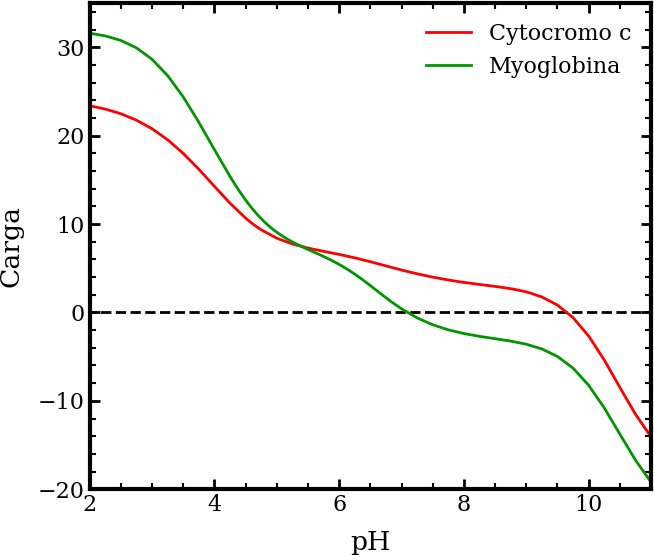
\includegraphics[width=0.9\textwidth]{Figures/graph-film/carga-proteinas.png}
    \caption{N\'umero de carga de las proteinas cytocromo c y myoglobina como  funci\'on del pH en el seno de la soluci\'on (bulk). La l\'inea a trazos muestra el cambio en el signo de la carga.}
    \label{fig:protein-charge}
\end{figure}



Sin embargo, aunque esto parece simplificar el problema de establecer la carga neta de cualquier especie dentro del material, incluida la red polim\'erica y las prote\'oinas adsorbidas, determinar los cambios en el pH local tiene la misma complejidad que el problema original (es decir, determinar la carga de la la red). El pH local que se establece dentro del material, as\'i como su valor en la interfaz entre el pol\'imero y la soluci\'on acuosa, es el resultado de la compleja interacci\'on entre la organizaci\'on molecular, los equilibrios qu\'imicos y las interacciones f\'isicas que determinan el equilibrio termodin\'amico a las condiciones impuestas externamente (pH, concentraci\'on de sal). Por ejemplo, la figura \ref{fig:pH-local} muestra el pH dentro de una pel\'icula de hidrogel de PMAA como una funci\'on del pH  y la concentraci\'on de sal, calculado usando teor\'ia molecular.

\begin{figure}
    \centering
    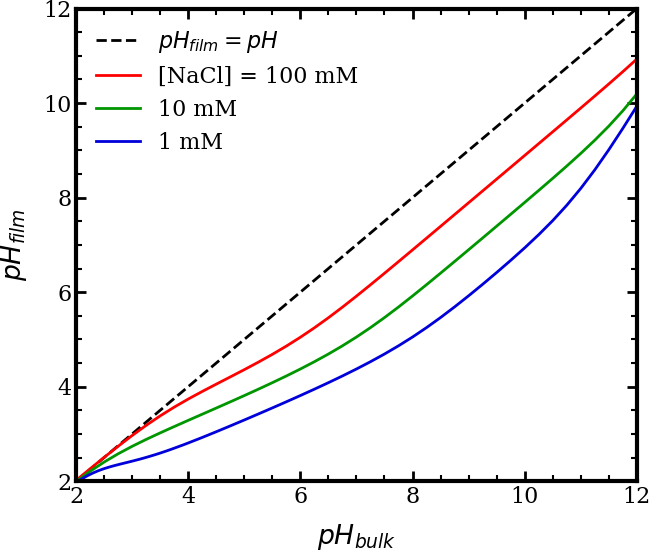
\includegraphics[width=0.9\textwidth]{Figures/graph-film/pH-local.png}
    \caption{pH local del gel como funci\'on del pH en el seno de la soluci\'on (bulk). Cada curva corresponde a una concentraci\'on de sal diferente.}
    \label{fig:pH-local}
\end{figure}

\subsection{Adsorci\'on}
Como se mencion\'o al incio de este capitulo... poder usar estos sistemas de hidrogeles como carries de adsrobatos de utilidad terap\'eutica.
Para ello nos valdremos de la teor\'ia molecular y haciendlo uso de ciertas prote\'inas modelo como lo son el cytocromo c y la myoglobina. estas dos presentan gran estabilidad en un amplio rango de pH y recientemente se ha  investigado la termodinámica  de su adsorci\'on en sistemas polim\'ericos similares. \addcite

Para cuantificar la cantidad de adsrobato adsrobido en el hidrogel utilizamos la expresi\'on:

\begin{align}
\Gamma = \int_V {dr(\rho(r) -\rho_{bulk}}  
\label{adsor}
\end{align}

en donde $\rho(r)$ y $\rho_{bulk}$ son las densidades del  locales y en el seno de la soluci\'on del adsorbato respectivamente, V es el volumen de la soluci\'on. 
Esta adsorci\'on proporciona la masa  en un volumen particular por exceso de la contribuci\'on del bulk. En particular dentro del hidrogel, $\Gamma$ proporciona la cantidad de adsorbato en exceso dentro del material, recibiendo tambi\'en contribuciones de la interfaz de soluci\'on de pol\'imero.

Para estas prote\'inas, la adsorci\'on es una funci\'on no monot\'onica del pH de la soluci\'on (ver Figura \ref{fig:ad-pro}). A pH bajo, estas prote\'inas tienen una carga alta y positiva, pero la red de poli\'acidos solo está d\'ebilmente ionizada (v\'eanse las Figuras \ref{fig:degree-film} y \ref{fig:protein-charge}). A un pH suficientemente alto, por otro lado, el pol\'imero est\'a fuertemente cargado negativamente, pero las prote\'inas tienen una carga d\'ebilmente positiva o incluso negativa. Bajo tales condiciones (muy) \'acidas o alcalinas, las interacciones electrost\'aticas son d\'ebilmente atractivas o repulsivas. No hay fuerza impulsora para la adsorci\'on. A valores de pH intermedios, por el contrario, donde tanto la prote\'ina como la red de poli\'acidos tienen cargas fuertes y opuestas, se produce una adsorci\'on significativa con un m\'aximo necesario en tales condiciones.

La adsorci\'on de prote\'inas depende cr\'iticamente de la concentraci\'on de sal de la soluci\'on. Este comportamiento se ilustra en la figura \ref{fig:ad-pro} que muestra la adsorci\'on de citocromo c  y mioglobina en una pel\'icula de hidrogel de PMAA. La disminuci\'on de las concentraciones de sal mejora la adsorci\'on y ampl\'ia el rango de pH de la adsorci\'on. Por ejemplo, ambos paneles de la \ref{fig:ad-pro} muestran una disminuci\'on de aproximadamente un orden de magnitud en la adsorci\'on cuando se comparan soluciones de NaCl 1 mM y 10 mM. El pH de m\'axima adsorci\'on tambi\'en depende de la salinidad de la soluci\'on. Este comportamiento es a\'un m\'as interesante cuando se considera que una concentraci\'on de sal m\'as baja conduce a una red con carga m\'as d\'ebil, como describimos con anterioridad. En otras palabras, la red de pol\'imero con carga m\'as d\'ebil, a medida que disminuye la concentraci\'on de sal, m\'as prote\'ina es adsorbida. Esta \'ultima afirmaci\'on es cierta en las concentraciones de prote\'ina ($10 \mu M$) y sal de la figura \ref{fig:ad-pro}, donde la adsorci\'on solo modifica ligeramente el grado de carga de la red.

Esta dependencia de la adsorci\'on de la concentraci\'on de sal tiene tres razones principales: en primer lugar, existe el apantallamiento  de las atracciones electrost\'aticas de la red hacia la prote\'inas por parte de los iones de sal. Cuanto menor sea la concentraci\'on de sal, m\'as débil ser\'a el apantallamiento de las interacciones prote\'ina-red, lo que mejora la adsorci\'on. En segundo lugar, a medida que la concentraci\'on de sal disminuye, el pH dentro de las gotas de hidrogel (a un pH general dado). Esto implica que las prote\'inas adsorbidas tienen una carga m\'as positiva tras la adsorci\'on (a medida que disminuye [NaCl]). En tercer lugar, la ganancia entr\'opica de la liberaci\'on de contraiones de la red de pol\'imeros es mayor a medida que disminuye la concentraci\'on de sal, lo que tambi\'en favorece la adsorci\'on de prote\'inas.



\begin{figure}
    \centering
    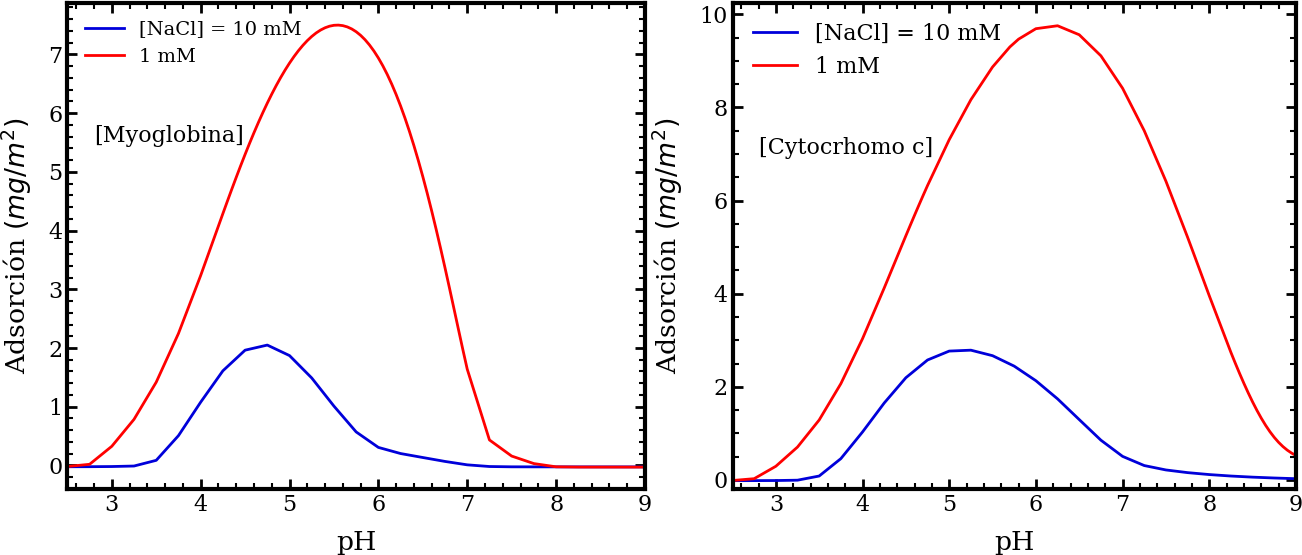
\includegraphics[width=0.99\textwidth]{Figures/graph-film/ad-proteins.png}
    \caption{Adsorci\'on de proteinas: cytocromo c y myoglobina en panel A y B respectivamente. La concentraci\'on de los adsorbatos es $10 \mu M$}
    \label{fig:ad-pro}
\end{figure}
